The ICARUS-T600 detector is the largest LArTPC experiment ever actualized containing 760 tons of purified liquid argon (476 tons of active mass). Comprised of two 300 ton modules, the T600 detector initially tested in Pavia, Italy in 2001 where one of the two modules was exposed to surface running for a three month period. Extensive system testing was performed before the complete system was transported to the underground Gran Sasso National Laboratories (LNGS). In 2010, the entire T600 detector was brought online at Gran Sasso where it completed a three year neutrino run in the Cern to Gran Sasso (CNGS) neutrino beam corresponding to $8.6 \times 10^{19}$ protons-on-target. The successful operation of a large LArTPC experiment in an underground facility with $>90\%$ data taking efficiency (collecting $\sim$3000 neutrino events) and achieving high argon purity and long argon lifetime represents a major technological milestone for LArTPC's.

In 2014 the ICARUS-T600 detector was decommissioned and transported to CERN to undergo a refurbishment and upgrade in anticipation of its future non-underground operation at Fermilab's SBN program. Figure \ref{fig:ICARUSTPC} shows one of the two TPC modules at CERN undergoing refurbishment. Each module in the ICARUS detector is comprised of a common cathode and a TPC with dimensions 18.0~m~$\times$~1.5~m~$\times$3.2~m (l$\times$w$\times$h). The TPC has three instrumented wire planes with the first two induction planes oriented at $\pm 60^{\circ}$ to the beam axis and the final plane oriented horizontally. Both the pitch and wire spacing is chosen to be 3~mm which provides superb resolution for imaging interactions inside the detector. 

\begin{figure}[htb]
\centering
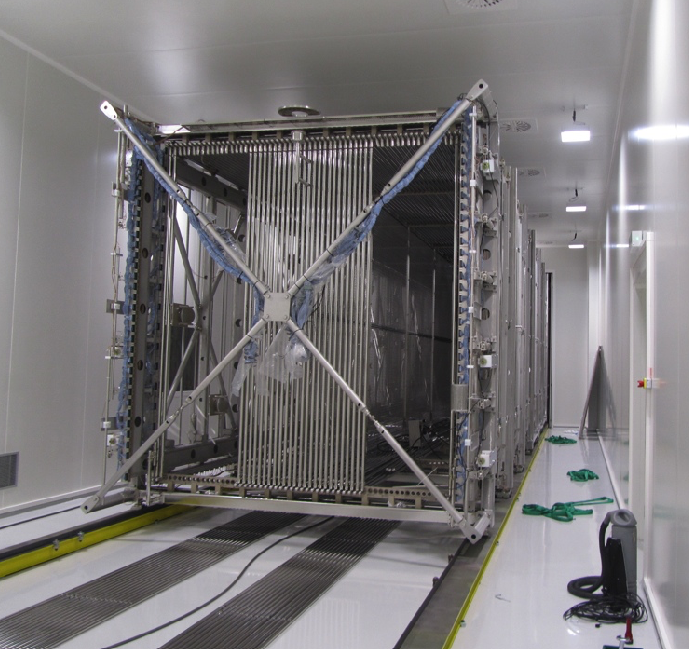
\includegraphics[width=0.50\textwidth]{images/ICARUSTPC.png}
\caption[]{An ICARUS TPC module located at CERN undergoing refurbishment in anticipation of the move to Fermilab in 2017-2018.}
\label{fig:ICARUSTPC}
\end{figure}

The importance of the ICARUS-T600 experiment to the experimental reach of the SBN program is shown in Figure \ref{fig:sense}. Plotted is the significance with which an experimental configuration covers the 99$\%$ confidence level (C.L.) for the allowed sterile neutrino mixing from the LSND experiment as a function of $\Delta m^{2}$ (the mass difference between the active and sterile neutrinos) for the simplest 3+1 model. The gray bands represent ranges of $\Delta m^{2}$ where LSND reports no allowed regions at 99$\%$ C.L. The presence of the ICARUS-T600, by providing a large sensitive mass at the far detector location, is absolutely imperative for the SBN program to achieve a definitive ($5\sigma$) coverage of the LSND allowed region.

\begin{figure}[htb]
\centering
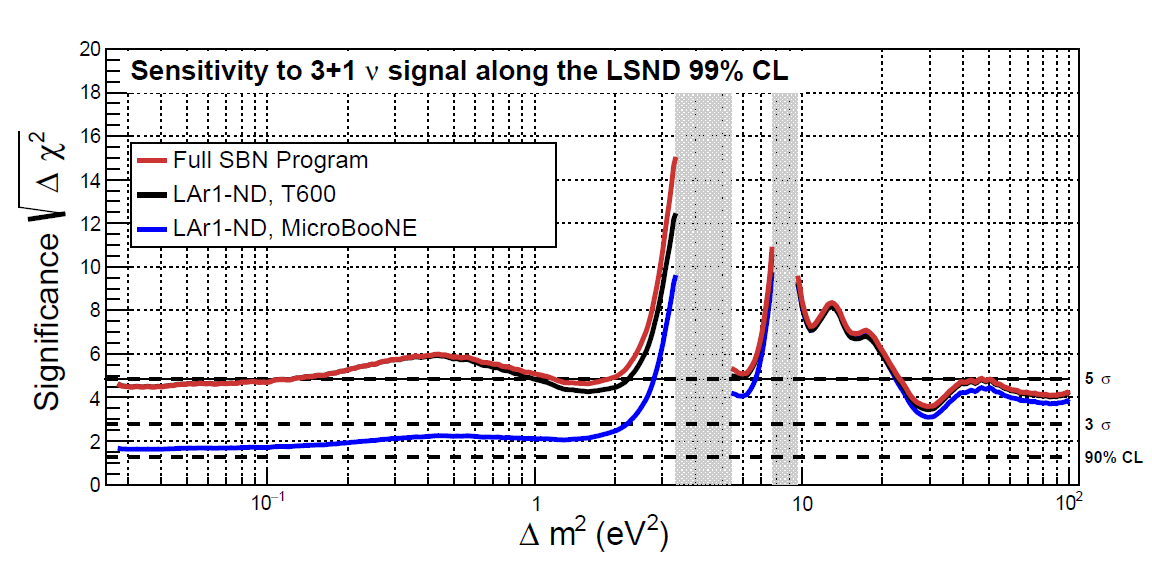
\includegraphics[width=0.78\textwidth]{images/Sensitivity.png}
\caption[]{The experimental sensitivity for $\nu_{\mu} \rightarrow \nu_{e}$ oscillations including backgrounds and systematics assuming a nominal three year exposure in the BNB for the SBND and ICARUS experiments and a six year exposure for the MicroBooNE experiment.}
\label{fig:sense}
\end{figure}


The UTA group has already begun contributing to the ICARUS experiment with the continued stationing of the post-doctoral researcher Andrea Falcone at CERN to continue his contributions to the upgrade of the ICARUS light detection system. The upgraded light detection system is currently being installed with 90-PMTs per TPC providing an estimated 5$\%$ photo-cathode coverage. The increased coverage will allow for excellent trigger efficiency for neutrino induced events as well as providing cosmogenic background rejection. Falcone is also leading the work to develop the readout electronics for the light detection system and integrating them into the common data aquisition system (artDAQ) used by the other two SBN experiments.


%%%%%%%%%%%%%%%%%%%%%%%%%%%%%%%%%%%%%%%%%%%%%%%%%%%%%%%%%%%%%%%%%%%%%
\subsubsection{Installation, and Commissioning}\label{sec:ICARUSBulid}
%%%%%%%%%%%%%%%%%%%%%%%%%%%%%%%%%%%%%%%%%%%%%%%%%%%%%%%%%%%%%%%%%%%%%
By participating in both the installation, commissioning, and data taking of the SBND and MicroBooNE as well as leveraging on the experience of Dr. Falcone's work on ICARUS already, the researchers supported by this proposal will be well positioned to contribute to the installation, commissioning, and first data analysis of the ICARUS LArTPC upon its arrival at Fermilab. Having a robust team of researchers based at Fermilab to provide expertise and support for the ICARUS system will ensure the successful execution of the SBN program.

Falcone is expected to travel with the ICARUS detector when it moves to Fermilab in early 2017 and play a key role in the commissioning and data acquisition of the light system. At the same time he will be training the other post-doctoral and graduate researchers on the ICARUS system to ensure a smooth first data taking in mid to late 2017. These detector experts are expected to remain in residence at FNAL during the initial operations of the detector and play a key role in early data analysis.

%%%%%%%%%%%%%%%%%%%%%%%%%%%%%%%%%%%%%%%%%%%%%%%%%%%%%%%%%%%%%%%%%%%%%
\subsubsection{ICARUS Data Analysis}\label{sec:ICARUSDataAnalysis}
%%%%%%%%%%%%%%%%%%%%%%%%%%%%%%%%%%%%%%%%%%%%%%%%%%%%%%%%%%%%%%%%%%%%%
In addition to providing the necessary sensitivity in the $\nu_{\mu} \rightarrow \nu_{e}$ oscillation channel, the large mass and long length of the detector allow for more complete containment of high energy muons and electromagnetic showers due to $\pi^{0} \rightarrow \gamma \gamma$ decays. Using this, and the deployment of a near detector in the BNB beamline, a complimentary sterile neutrino search looking for muon neutrino disappearance as well as neutral current disappearance becomes possible. The extended length of the ICARUS-T600 detector provides better $\pi / \mu$ separation (since pions have a higher cross-section to interact) as well as more accurate muon energy reconstruction (since more muons will be fully contained) thus extending the sensitivity in the muon disappearance channel. 

Similarly, by targeting a clearly identifiable neutral current process (such as NC$\pi^{0}$ production) the disappearance rate can be measured at both the near and far detector to search for the sterile neutrino signature in a complimentary way to the $\nu_{e}$ appearance. ICARUS's large volume ensures near complete photon shower containment and thus increases the statistics available for a NC$\pi^{0}$ disappearance search.

On top of the three detector SBN program, the stand-alone T600 detector can offer physics insight through the study of neutrino cross-sections at energies pertinent to the future planned Deep Underground Neutrino Detector (DUNE). The ICARUS experiment can due this because it will see a significant off-axis component of the Neutrinos from the Main Injector (NuMI) beam. The NuMI beam uses 120 GeV protons to produce a higher energy neutrino beam than the BNB. ICARUS is expected to collect one neutrino event every 150 seconds from the NuMI beam in the energy range of 0-3~GeV. Such high energy neutrino cross-section data on an argon target will provide valuable input to the DUNE experiment and offer experimental measurements of detector efficiencies and event reconstruction techniques at these higher energies.

